\section{Encryption at Line Rate: How Fast do we need?}
\label{sec:crypto}

The attack demonstrated in Sec.~\ref{sec:poc.attack} suggests the necessity of encryption for RDMA traffic.
However, applications using RDMA aim for high speed network links running at typically 40 to 100 Gbps.
The RDMA traffic among machines is transferred in raw bytes without any encryption nowadays.
This is an obvious but unconsidered tradeoff between performance and security guarantees.
There are, as we believe, more balanced solutions in the design space of a secure and performant RDMA system.
In this section, we are going to discuss the encryption rate we need to support high-speed RDMA traffic
as the first step toward it.

An ideal implementation for RDMA encrypted traffic should be very similar to TLS that implemented on top of the transport protocols. It should be able to operate at line-rate of the underlying network. As the link rate of network soars over the last few years, we can easily purchase 200 Gbps off-the-shelf network interface cards supporting RDMA. However, the encryption rate grows slower than this though having instruction-level support on CPU, e.g. AES-NI on Intel x86 processors. We conducted a brief evaluation of encryption rate using common encryption algorithms and commodity CPUs. We chose to evaluate on block cipher, e.g. AES-CBC and AES-GCM and stream cipher, e.g. ChaCha20 with Poly1305. The evaluation executed on different block size ranging from 16 bytes to 8192 bytes. We ran encryption algorithms of OpenSSL 1.1.0 on a Intel Xeon E5-2650 v4 processor. It is single-threaded and with AES-NI enabled.

As Fig.~\ref{fig:cpu_encryption_rate} shown, the fastest AES-128-GCM encrypts 8k blocks around 26 Gbps which is way slower than the expected link rate of high speed network. Another downside of performing encryption on CPU is the waste of compute resources. CPUs are suppose to perform real computation instead of encryption. If we want to encrypt our data for RDMA traffic in 200 Gbps, then we need 8 physical cores dedicated for encryption. A server in datacenters usually has around 20 cores, and spending 8 cores dedicated for encryption is wasting 40\% of the compute power.

\begin{figure}[ht]
    \centering
    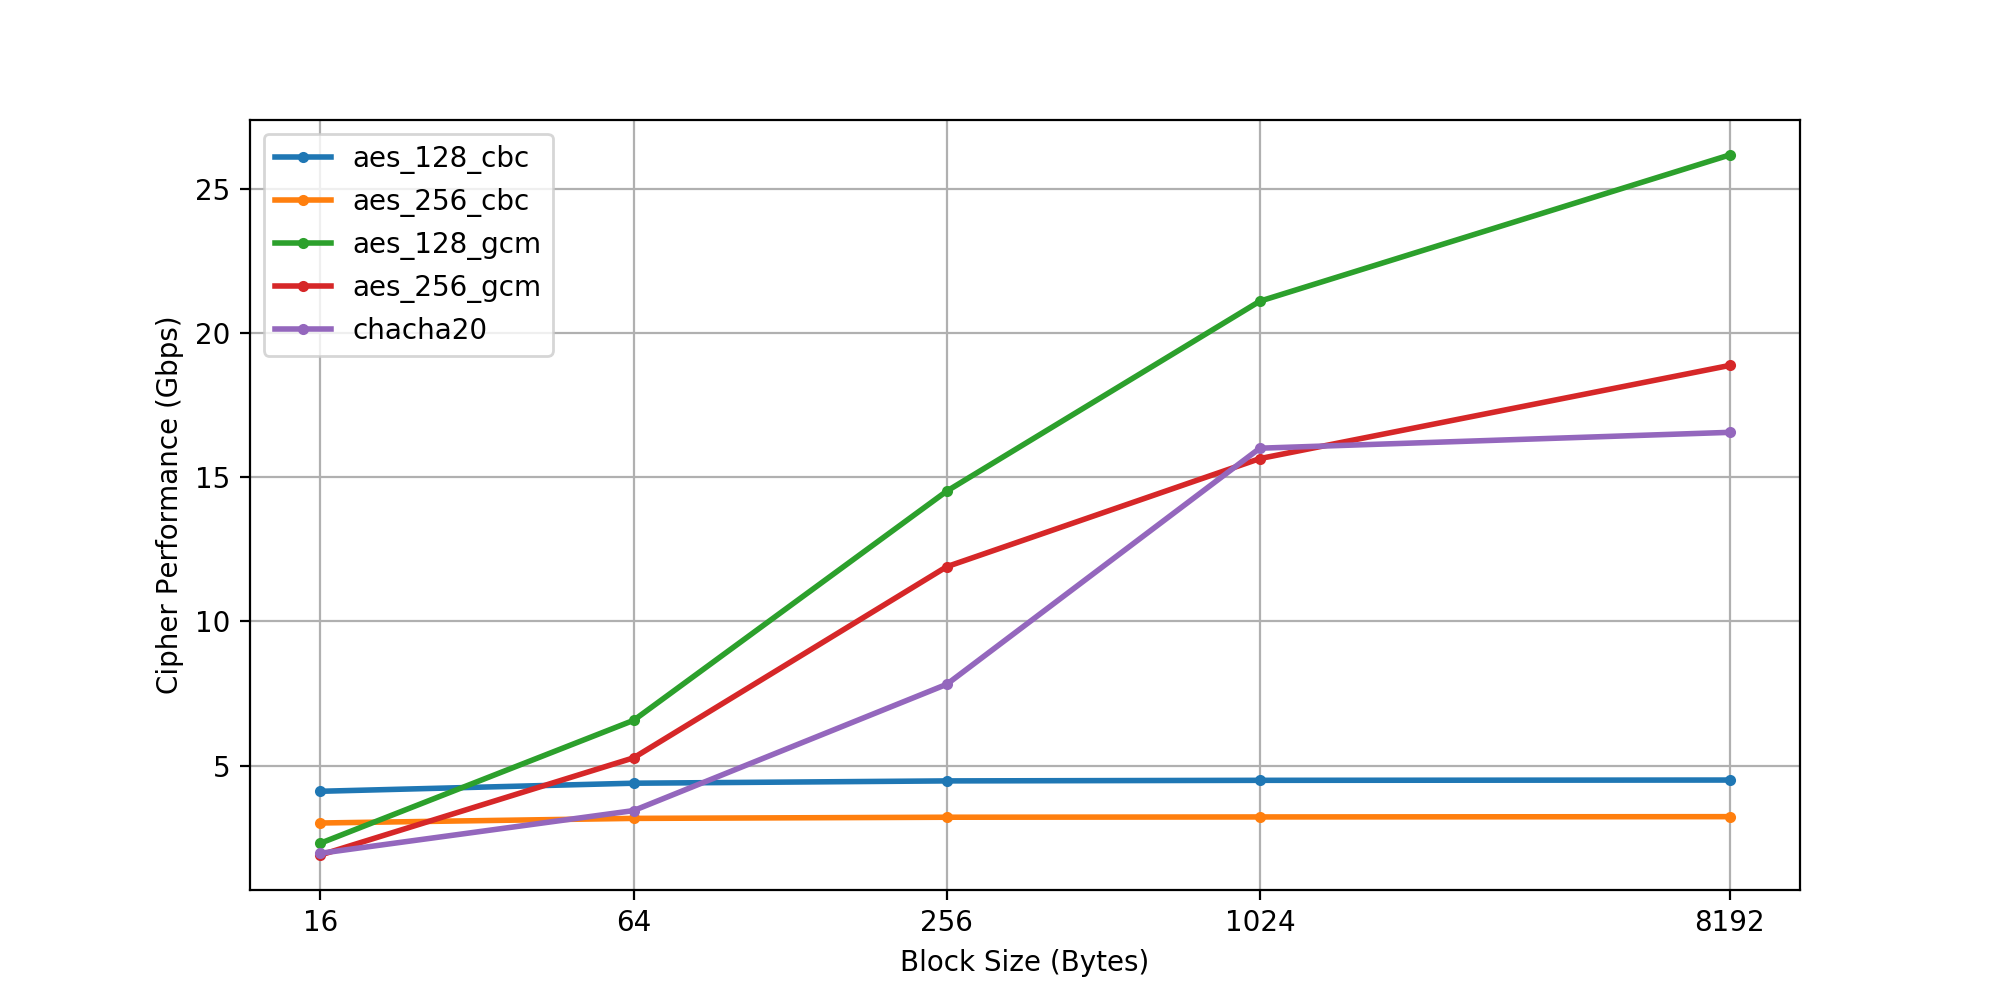
\includegraphics[width=0.55\textwidth]{fig/encryption}
    \caption{The encryption rate of an Intel CPU}
    \label{fig:cpu_encryption_rate}
\end{figure}

The result shown in Fig.~\ref{fig:cpu_encryption_rate} demonstrates the infeasibility of using CPU for encryption. We believe that offloading encryption onto network interface card is necessary. Cavium LiquidIO network interface card operate at 25 Gbps with a single 25 Gbps SerDes device. It can encrypt data close to its 25 Gbps line rate as it shown in Cavium's datacenter security white paper. It supports major encryption and HMAC algorithms, e.g. AES-CBC for 128, 192 and 256 bits, AES-GCM for 128, 192 and 256 bits, HMAC-MD5, HMAC-AES-XCBC, HMAC-SHA1, HMAC-SHA for 256, 384, and 512 bits. As faster network interface cards, e.g. 100 Gbps and 200 Gbps, are consist of multiple 25 Gbps SerDes devices, we expect to observe similar encryption rate. In addition, Mellanox ConnectX-6 200 Gbps network interface card supports XTS-AES for 256 and 512 bits key. It targets storage traffic, but its serves as another strong evidence for encryption offloading on network interface cards.
